\chapter{Experimental Evaluations}

The main objective of the study was to compare how close the values from the low cost sensor network is to that of the reference system which is placed at the Plaza 400 building, downtown Prince George. The sensor system was deployed for six days from 30 May,2019 to 4 June, 2019 and was later compared to the values from referance system. In this chapter we will be discussing on the nature of the values and how close are these values to that of the reference system.

\section{Deployment}

In order to understand the accuracy and precison of our system, we deployed the air pollution monitoring system for six days in University Heights, Prince George. The figure \ref{deployed} shows the experimental set up of the sensor system deployed at the location. The system was directly connected to a power code and was made to hung over a platform. The collected values were transferred to the ThingSpeak database through the WiFi module (Wemos) in an hourly averaged form and hence 24 data set points were collected for each day.

\begin{figure}[h]
    \begin{center}
    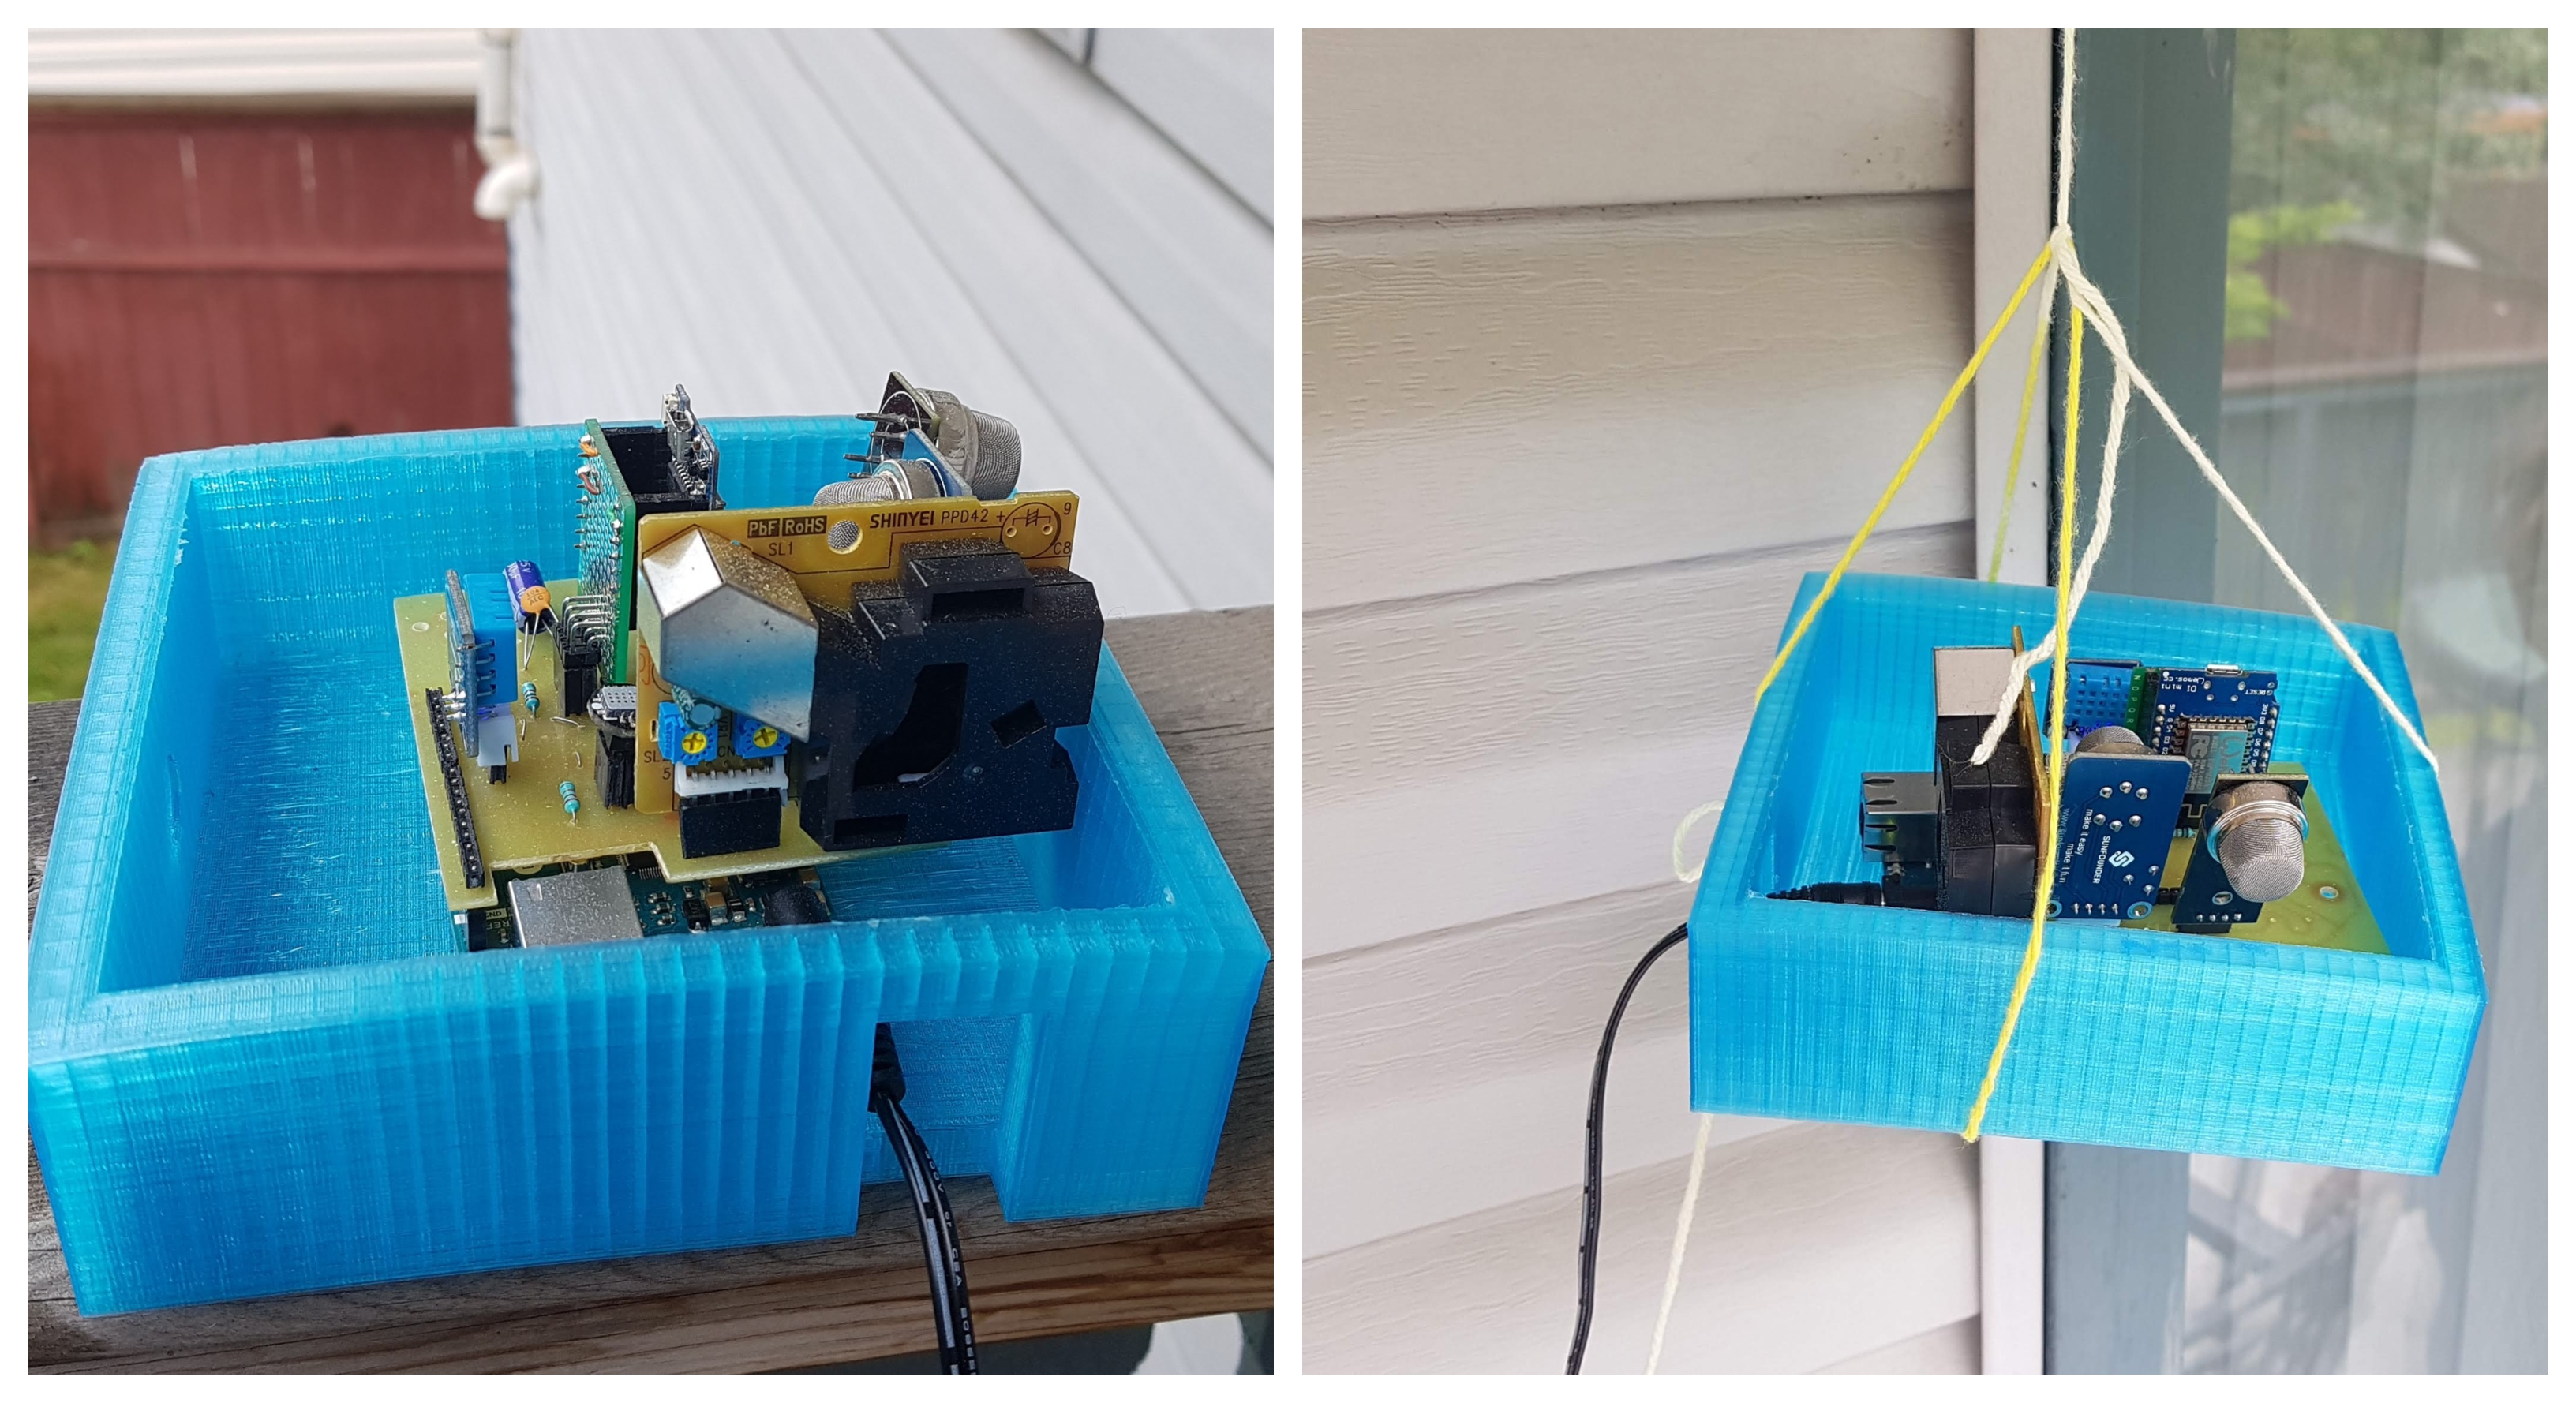
\includegraphics[scale=0.5]{images/figure20.jpg}
    \end{center}
    \caption{Deployed System at University Heights, Prince George}
    \label{deployed}

  \end{figure} 


  The main reason to conduct our deployment in this location was to have an easy access and to check on the system regularly in case of any sensor faults or signal distortions. The collected values in ThingSpeak database were compared to the reference values located in downtown Plaza 400 building except of carbon monoxide. The reference values for carbon monoxide were not found and hence were not analyzed. We have tried to analyze the daily variation of  Ozone, Particulate matter (both $PM_{2.5}$ and $PM_{10}$), Nitrogendioxide, temperature and humidity to their reference value.

  \section{Data Analysis}
  In this section we will be comparing the collected data for each sensors anw will be looking at the accuracy of these values. We will be using multiple line graph plots to observe the data and will be investigating if there is any variations to these data.
  \subsection{Ozone}

  The ground level ozne which is three atoms of oxygen ($O_3$) is measured with the help of a semiconductor sensor MQ 131 which changes its conductivity with ozone \cite{technicalsheetozone}. The content of Ozone gas during the day time is generally high due to the presence of other pollutant and is low during night. It can be seen from the graphs that our sensor was able to follow the trend similar to that of the reference system. In figure \ref{Ozone} shows the line graphs of the first three days of the experiment and it can be seen that the values are very close to the refernce system. This shows that the sensor gives very close value to reference system soon after calibration.


  
\begin{figure}[h]
    \begin{center}
    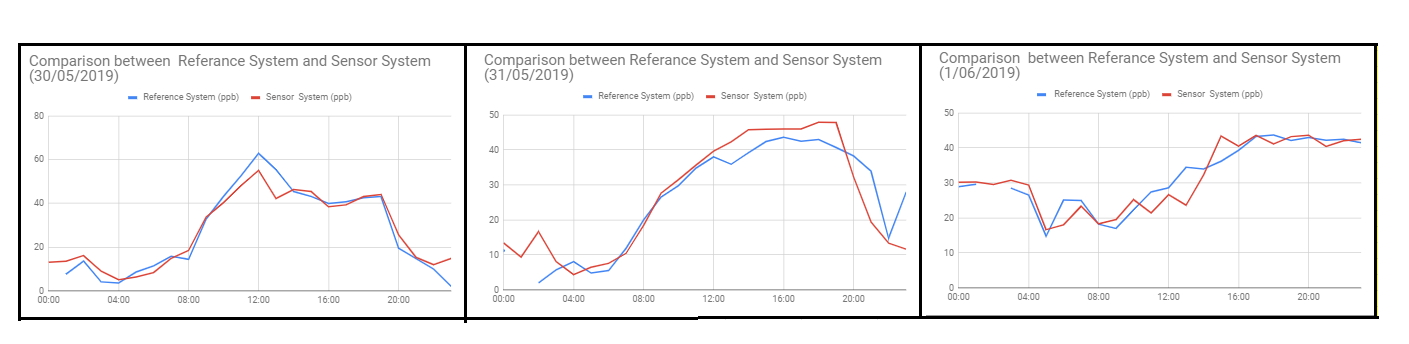
\includegraphics[scale=0.70]{images/figure21.png}
    \end{center}
    \caption{Comparison between Ozone values from sensor system and reference system from 30/05/2019 to 01/06/2019}
    \label{Ozone}

  \end{figure}
  \bigskip

In the next figure \ref{Ozone1} shows the graphs for the next three days and it can be clearly seen that on the last two days the values from the sensor shows a drastic variation. This can be interpreted in two ways either it could be because the system needs to be recalibrated. The system might need to be updates with new regression equation so as to provide the graphs similar to the reference system. Secondly, we can also interpret this as a location specific effect. As the reference system is in downtown and there is a possibility of some activity which can cause a change in values or vice versa.
  



\begin{figure}[h]
    \begin{center}
    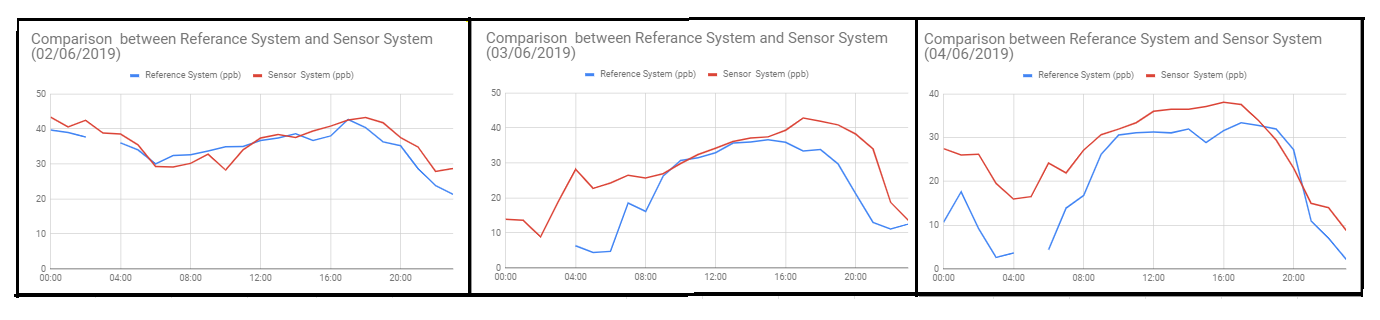
\includegraphics[scale=0.70]{images/figure22.png}
    \end{center}
    \caption{Comparison between Ozone values from sensor system and reference system from 02/06/2019 to 04/06/2019}
    \label{Ozone1}

  \end{figure}

  \bigskip

   Considering the fact that we are using a low cost sensor to measure the values from the air the need for calibration should be considered as a priority.


   \subsection{Nitrogen Dioxide}

   Another pollutant which we measured with sensor is oxides of Nitrogen which is generated from liberation of Nitrogen present in the fuels and is considered as a serious pollutant in the environment \cite{Salonen2019} \cite{govcanada}. This pollutant was measured with the help of a popular silicon gas sensor called as MICS-2714 by calculating the sensing resistance. The referance system located in Prince George plaza 400 is API $NO_{x}$ monitor \cite{Environment2010} which uses chemiluminesence principle to measure . The figure \ref{Nitrogen} and \ref{Nitrogen1} shows the graphical measurement values of the sensor in comparison with the reference system. 


   \begin{figure}[h]
      \begin{center}
      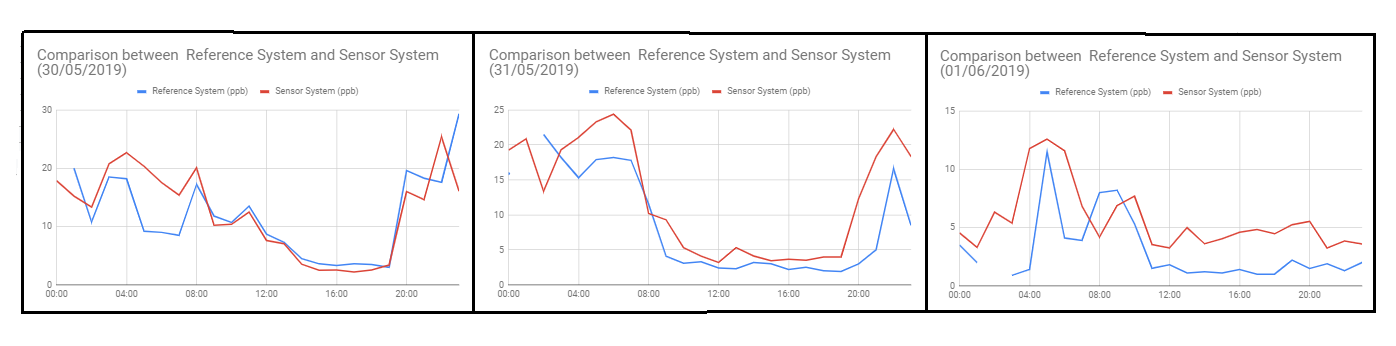
\includegraphics[scale=0.70]{images/figure23.png}
      \end{center}
      \caption{Comparison between Nitrogen Dioxide values from sensor system and reference system from 30/05/2019 to 01/06/2019}
    \label{Nitrogen}
  \end{figure}


  \bigskip

  It can be interpreted from the graph that even though the values of the pollutant at each point of time is different from the referance system but for the first three days the trend is followed. At the same time it can also be seen in the figure \ref{Nitrogen1} that the values from both the system have less similarity.

    \begin{figure}[h]
      \begin{center}
      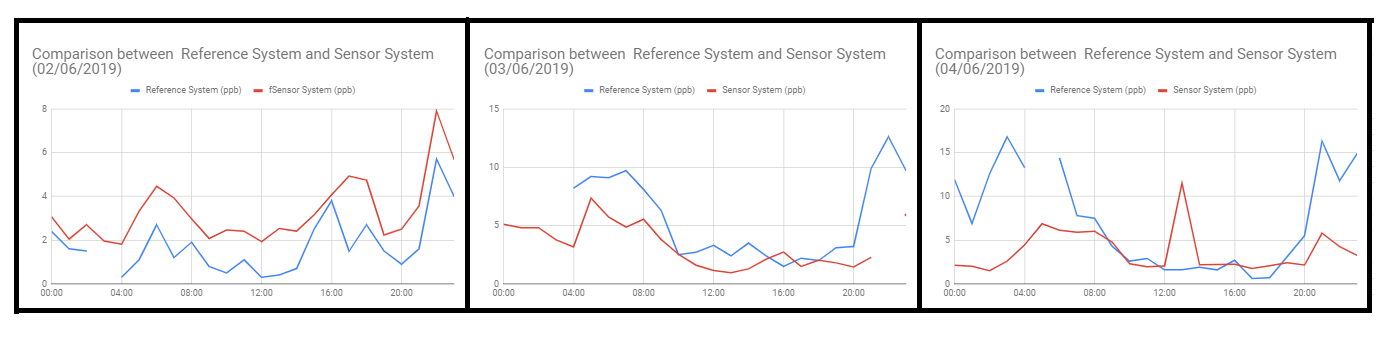
\includegraphics[scale=0.70]{images/figure24.png}
      \end{center}
      \caption{Comparison between Nitrogen Dioxide values from sensor system and reference system from 02/06/2019 to 04/06/2019}
      \label{Nitrogen1}
    \end{figure}

    

    It can be clearly seen from the graphs that the concentration of the Nitrogen oxide are high in the morning and then the slope comes down and again rises in the night. This variation of Nitrogen oxide can be because of less or no  solar radiation in the early morning and late night \cite{Environment2010} \cite{George2005}. The less amount of energy from sun slows down the breakdown of Nitrogen Oxide to Nitric oxide which inturn increses the amount of Nitrogen oxides in the stratosphere \cite{EnvironmentalQualitySectionMoE2012} \cite{Environment2010}. This can be clearly seen in the graphs in both referance value as well as in our sensor value. Another resaon for high values can also be related to heavy traffic as in the graph it clearly shows the concentration hits its peak around 8.00 am which is considered as an office time for most people in the city. The results from our observation shows that our sensor only shows the best measurement for the first two days and later the fluctuation in the concentration is high. This can be due to less sensitivity of the sensor used for measurement or might need better calibration method for the system.



\subsection{Particulate Matter}

The Particulate matters are those particles whose size ranges from 0.001$um$ till 100 $um$. The sources for the generation of this pollutant varies from town to town. In Prince George, pulp mills and saw mills are the primary soucrce for their emission and during winter road dust also adds to the primary pollutant category as winter street sanding is done around that time \cite{Champagne1996}.


    \begin{figure}[h]
      \begin{center}
      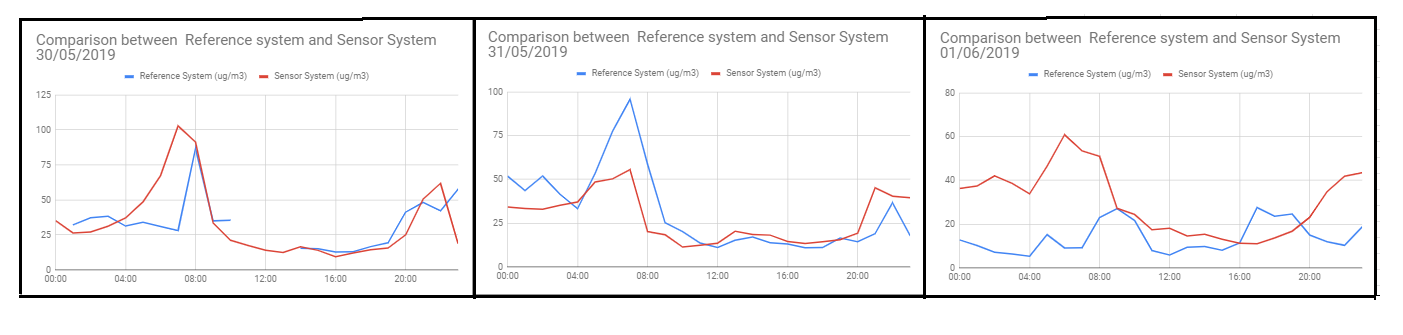
\includegraphics[scale=0.70]{images/figure25.png}
      \end{center}
      \caption{Comparison between $PM_{10}$ values from sensor system and reference system from 30/05/2019 to 01/06/2019}
    \label{PM10}
  \end{figure}

  
  \begin{figure}[h]
    \begin{center}
    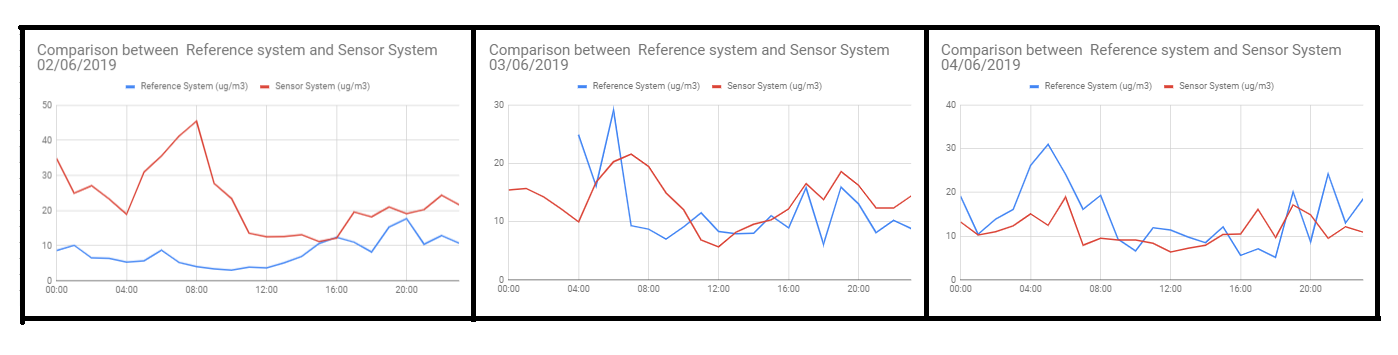
\includegraphics[scale=0.70]{images/figure26.png}
    \end{center}
    \caption{Comparison between $PM_{10}$ values from sensor system and reference system from 02/06/2019 to 04/06/2019}
    \label{PM101}
  \end{figure}

  
  \begin{figure}[h]
    \begin{center}
    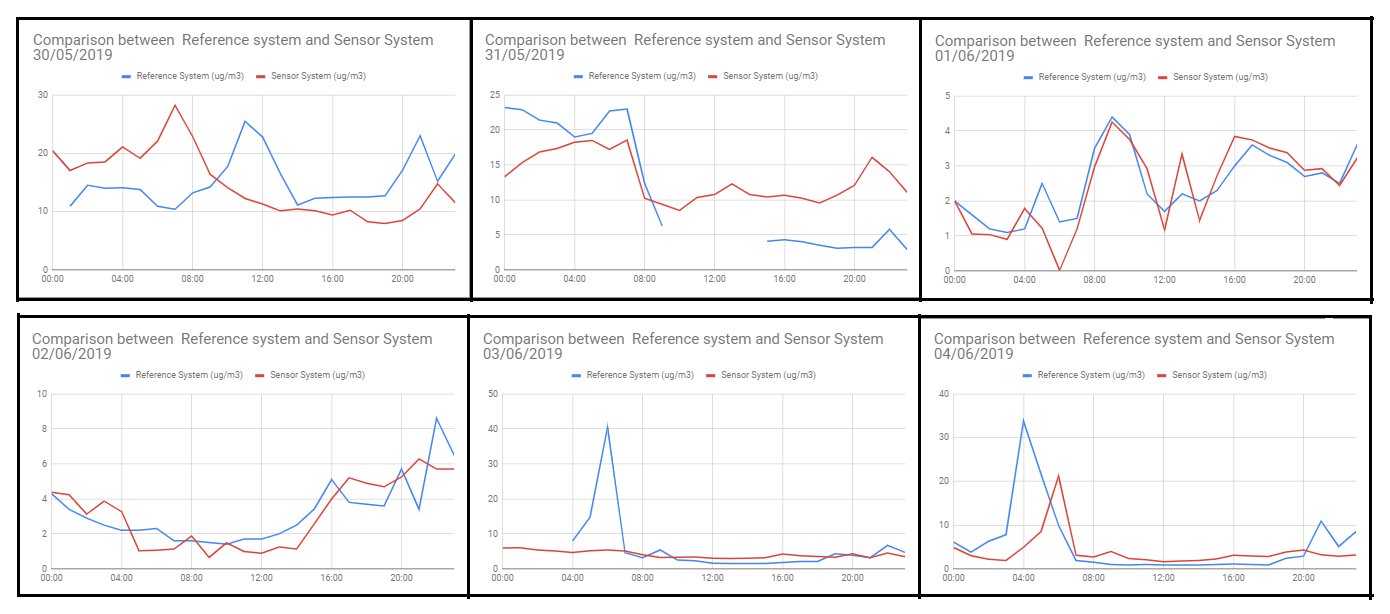
\includegraphics[scale=0.70]{images/figure27.png}
    \end{center}
    \caption{Comparison between $PM_{2.5}$ values from sensor system and reference system from 30/05/2019 to 01/06/2019}
  \label{PM2.5}
\end{figure}

\begin{figure}[h]
  \begin{center}
  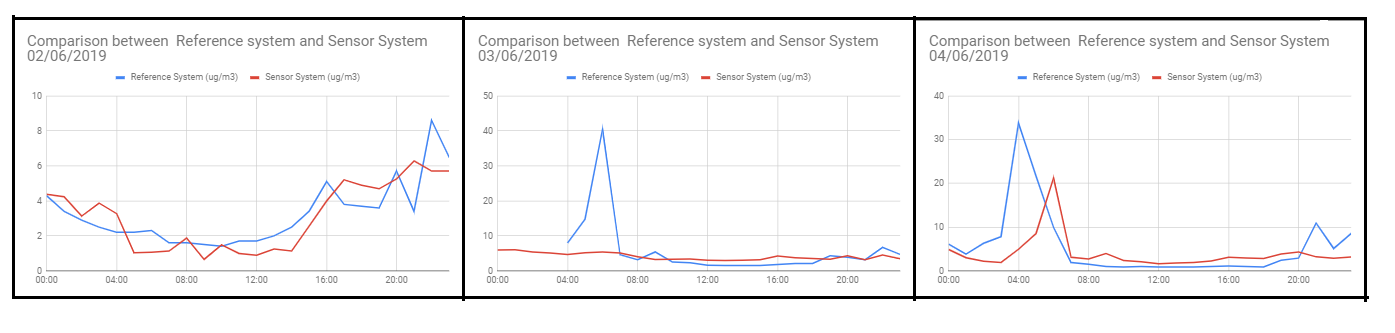
\includegraphics[scale=0.70]{images/figure28.png}
  \end{center}
  \caption{Comparison between $PM_{2.5}$ values from sensor system and reference system from 02/06/2019 to 04/06/2019}
  \label{PM2.51}
\end{figure}







